\documentclass{article}
\usepackage[utf8]{inputenc}
\usepackage{caption}
\usepackage[margin=1in]{geometry}
\usepackage{graphicx}
\usepackage{pdfpages}
\pdfminorversion=7

\begin{document}
\begin{titlepage}


\centering
\vspace*{2cm}
{\Huge User Interface Design Document\par}
\vspace{.25cm}
{\LARGE Course Evaluation System\par}
\vspace{1cm}
{\Large Team EVAL\par}
\vspace{.2cm}
{\Large Jovon Craig, Sam Elliott, Robert Judkins, and Stanley Small\par}
\vspace{1cm}
{\Large Client: Dr. Harlan Onsrud\par}
\vspace{1cm}
{\Large November 30, 2018\par}
\vspace{11cm}

University of Maine - Fall of 2018 - COS 397

Instructor: Professor Terry Yoo

\end{titlepage}

\newpage

\begin{center}
{
\includegraphics[scale=.2]{images/team_logo.png}} \\ 	\bigskip
{\LARGE Course Evaluation System } \\ \medskip
{\large User Interface Design Document } \\ \medskip
\end{center}

\tableofcontents

\newpage

\section{Introduction}
 

\subsection{Purpose of This Document}

This user interface design document is an overview of the graphics and layouts shown to the users of our course evaluation system. The first section, the user interface standards, describes the general features of the graphics, such as layouts and components that are common to all screens in the interface. The second section, the user interface walkthrough, includes a ``navigation diagram'' of the order in which the screens are shown, and complete wireframes of each screen. The docuement's third section gives the data items typically entered in the user interface and how they are formatted.

This document is intended for the development team, the product client, Dr. Harlan Onsrud, and potential users of the system. Team EVAL needs this document to properly implement the user interface in code. Dr. Onsrud also needs it to verify that the program's appearance looks appropriate for universities and to suggest revisions to the UI. Lastly, the document helps the software's users, serving as a guide on how to use the software.


\subsection{References}

Craig, J., Elliott, S., Judkins, R., \& Small, S. 29 October 2018. \textit{System Requirements Specification.}
\vspace{3mm}\newline
Craig, J., Elliott, S., Judkins, R., \& Small, S. 16 November 2018. \textit{System Design Document.}
\vspace{3mm}\newline
Onsrud, H. ``Example Question Selection Form.'' See Appendix D.

\section{User Interface Standards}

Figure 1 is the overall screen layout of our course evaluation system. It shows the general areas and components of each screen in the interface and how the user will navigate through the screens.

\section{User Interface Walkthrough}

Figure 2 is a diagram that shows the paths that a user can take to navigate the system's interface. It also includes the names for all the screens in the UI.

The next set of figures is the wireframes for each screen in the evaluation system. These diagrams are meant to communicate the areas, menus, and buttons that are unique to a certain screen and what they do.


\section{Data Validation}

The following table lists each data item in the user interface of the evaluation system. A data item is an input that a user enters into the system and has a specified format.

\begin{center}
\captionof{table}{Data item specification}
\begin{tabular}{|p{3cm}|p{1.8cm}|p{2cm}|p{2cm}|p{4cm}|} 
\hline
\textbf{Label} & \textbf{Screen(s)} & \textbf{Data Type} & \textbf{Format} & \textbf{Limit(s)} \\
\hline
 & & & & \\ 
\hline
 & & & & \\ 
\hline
 & & & & \\ 
\hline
 & & & & \\ 
\hline
 & & & & \\ 
\hline
 & & & & \\ 
\hline
 & & & & \\ 
\hline
 & & & & \\ 
\hline
 & & & & \\ 
\hline
 & & & & \\ 
\hline
\end{tabular}
\end{center}

\section{Report Formats}


\appendix

\newpage
\section{Agreement Between Customer and Contractor}
This page shows that all members of Team EVAL and the client, Harlan Onsrud, have agreed on all the information in the user interface design document. By signing this document, Team EVAL and Dr. Onsrud approve all of the designs for each screen in the interface, as well as how to navigate the interface.

The team will follow a process in the case that the design document is changed after we sign it. First, the team will write a rough draft of the changes to be made to the document. Second, all team members and Harlan Onsrud will sign the document agreeing to the changes. Finally, the team will make the changes to the final copy of the document.

\vspace{.7in}
\noindent
\begin{tabular}{ p{5cm} p{5cm} p{5cm} } 
\textbf{\textit{Name}} & \textbf{\textit{Signature}} & \textbf{\textit{Date}} \\[.5cm]
\textbf{Jovon Craig} & $\rule{5cm}{.1mm}$ & $\rule{5cm}{.1mm}$\\[.5cm]
\textbf{Sam Elliott} & $\rule{5cm}{.1mm}$ & $\rule{5cm}{.1mm}$\\[.5cm]
\textbf{Robert Judkins} & $\rule{5cm}{.1mm}$ & $\rule{5cm}{.1mm}$\\[.5cm]
\textbf{Stanley Small} & $\rule{5cm}{.1mm}$ & $\rule{5cm}{.1mm}$\\[.5cm]
\textbf{Harlan Onsrud} & $\rule{5cm}{.1mm}$ & $\rule{5cm}{.1mm}$\\[.5cm]
Customer Comments: & \multicolumn{2}{ l }{ $\rule{10.45cm}{.1mm}$ }\\[.5cm]
\multicolumn{3}{ l }{ $\rule{15.9cm}{.1mm}$ }\\[.5cm]
\end{tabular}

\newpage
\section{Team Review Sign-off}

This page shows that all members of Team EVAL have reviewed the user interface design document and agreed on its content. By signing this document, the team members agree that all information about the evaluation system's UI is accurate, and that there is nothing in the document that is a source of contention.

\vspace{.7in}
\noindent
\begin{tabular}{ p{5cm} p{5cm} p{5cm} } 
\textbf{\textit{Name}} & \textbf{\textit{Signature}} & \textbf{\textit{Date}} \\[.5cm]
\textbf{Jovon Craig} & $\rule{5cm}{.1mm}$ & $\rule{5cm}{.1mm}$\\[.5cm]
Comments: & \multicolumn{2}{ l }{ $\rule{10.45cm}{.1mm}$ }\\[.5cm]
\multicolumn{3}{ l }{ $\rule{15.9cm}{.1mm}$ }\\[.5cm]
\textbf{Sam Elliott} & $\rule{5cm}{.1mm}$ & $\rule{5cm}{.1mm}$\\[.5cm]
Comments: & \multicolumn{2}{ l }{ $\rule{10.45cm}{.1mm}$ }\\[.5cm]
\multicolumn{3}{ l }{ $\rule{15.9cm}{.1mm}$ }\\[.5cm]
\textbf{Robert Judkins} & $\rule{5cm}{.1mm}$ & $\rule{5cm}{.1mm}$\\[.5cm]
Comments: & \multicolumn{2}{ l }{ $\rule{10.45cm}{.1mm}$ }\\[.5cm]
\multicolumn{3}{ l }{ $\rule{15.9cm}{.1mm}$ }\\[.5cm]
\textbf{Stanley Small} & $\rule{5cm}{.1mm}$ & $\rule{5cm}{.1mm}$\\[.5cm]
Comments: & \multicolumn{2}{ l }{ $\rule{10.45cm}{.1mm}$ }\\[.5cm]
\multicolumn{3}{ l }{ $\rule{15.9cm}{.1mm}$ }\\[.5cm]
\end{tabular}


\newpage
\section{Document Contributions}

Stanley Small ?? Stan contributed approximately ?? percent of the document.


Jovon Craig ??. Jovon contributed about ?? percent of the document.


Sam Elliott ??. Sam contributed about ?? percent of the document.

Robert Judkins ??. Robert contributed about ?? percent of the document.

\newpage

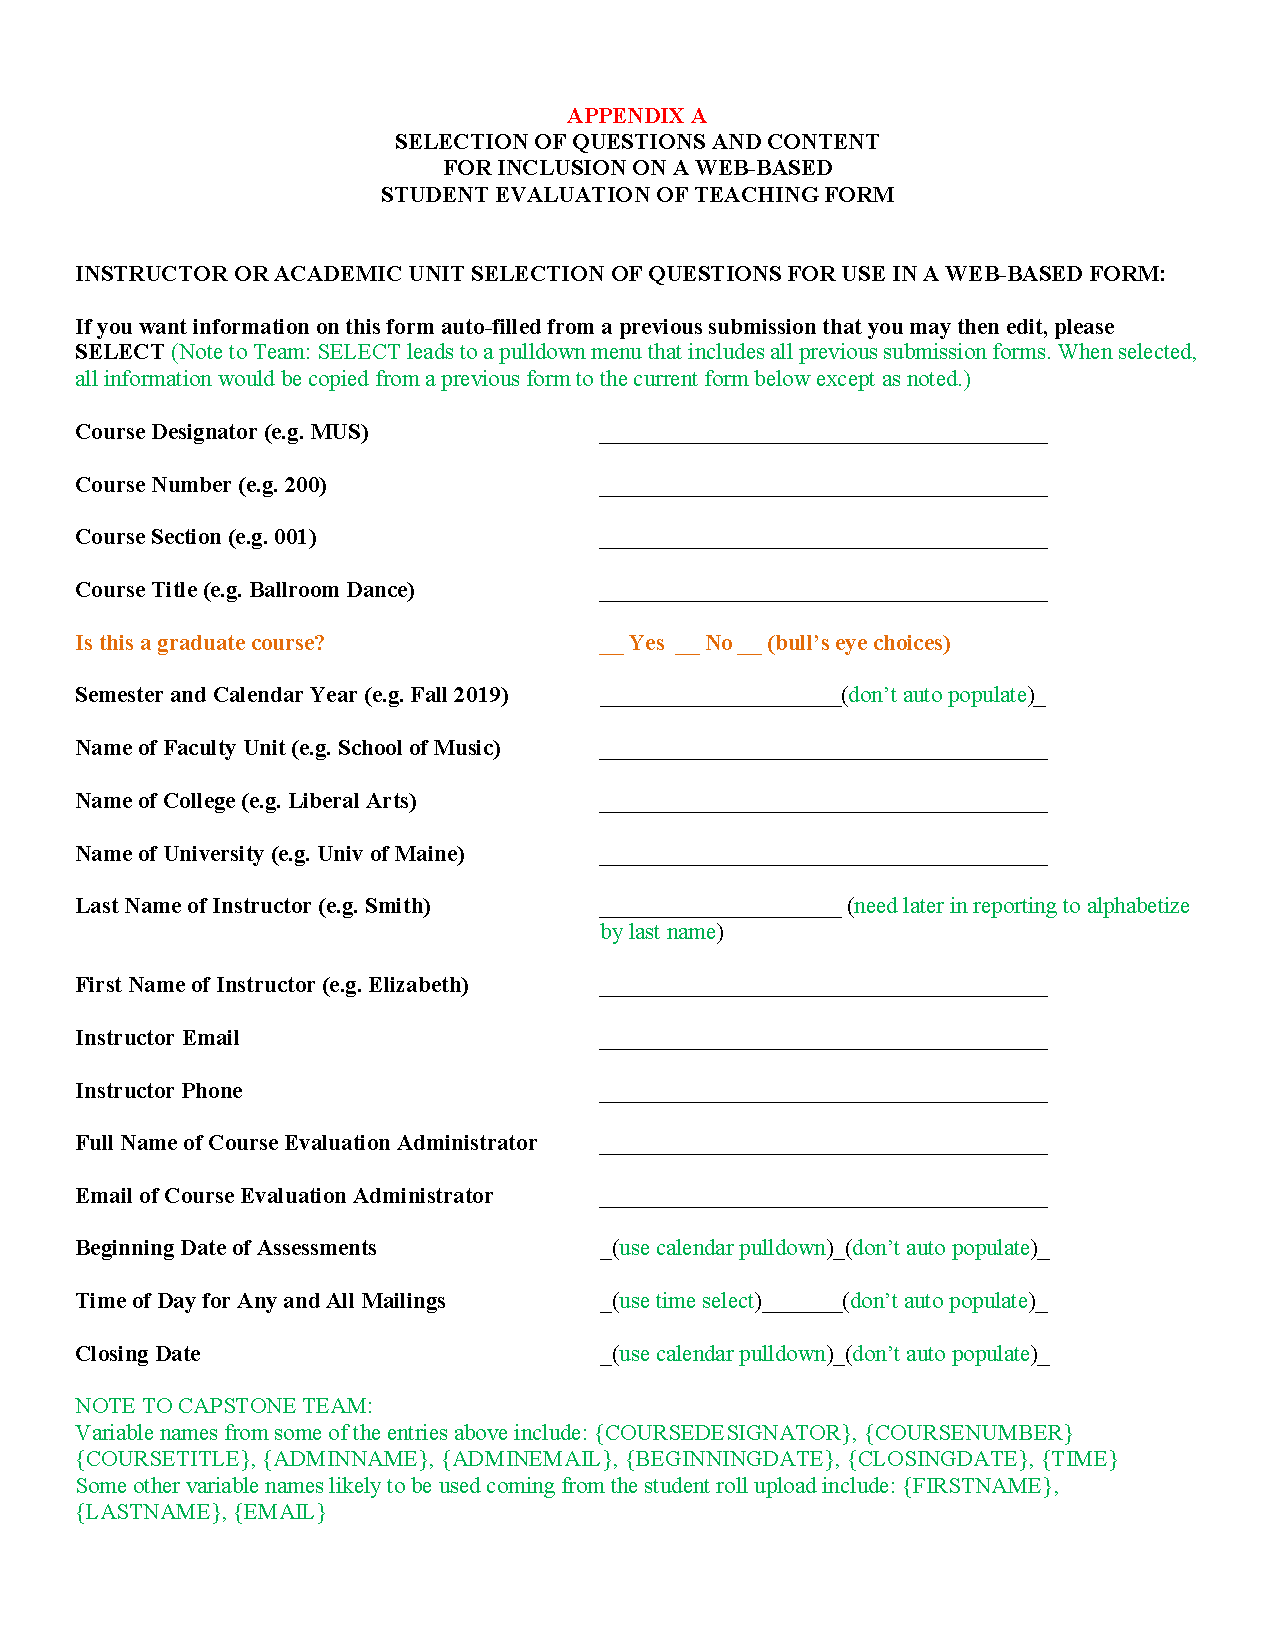
\includepdf[scale=0.85,pages=1,pagecommand=\section{Example Question Selection Form}]{images/question_appendix.pdf}
\includepdf[scale=0.85,pages=2-]{images/question_appendix.pdf}

\end{document}
